\section{Introduction}
Large-scale penetrations of smartphones across different corners of the world have made the personalized live video streaming applications very popular; according to Sandvine 2019 Mobile Internet Phenomena Report\footnote{\url{https://www.sandvine.com/2019-mobile-internet-phenomena-report} (last accessed: \today)}, YouTube contributes to $35\%$ of the global mobile Internet traffic, whereas applications like Facebook video, Instagram and NetFlix are constantly gaining popularity.  At the same time, various interesting live streaming applications are getting boosted up, such as Twitch.tv~\cite{pires2015youtube} where the users form various gaming communities to stream live gaming videos among themselves. Several other mobile live streaming applications are in place, such as Periscope and Meerkat. With all these applications where users share live videos among themselves, and such videos contribute a majority of the Internet traffic, one major question is how we can make the streaming effective while contributing less to the global mobile Internet traffic. 

Video streaming applications, including live streaming, mostly use Dynamic Adaptive Streaming over HTTP (DASH)~\cite{stockhammer2011dynamic} primary because of two reasons. (1) It provides a robust client-driven methodology to adapt the video quality based on the available network bandwidth, reducing the re-buffering and hence, improving the quality of experience (QoE) for the end-users. (2) Internet is full of middle-boxes like network address translation (NAT) and proxies; DASH can work perfectly over such middle-boxes. Adapting the video quality level during a live streaming is more challenging compared to the same for a buffered streaming; however, recent researches~\cite{TNET-Migration-2016,huysegems2015http,roverso2015smoothcache,merani2016adaptive} have developed various technologies to support adaptive live streaming over the Internet. However such dynamic adaptation techniques for live videos either (a) require complex time-consuming encoding methods such as Scalable Video Coding (SVC), or (b) take third-party supports such as a cloud-assisted live streaming to the peers. 

In this work, we develop a system for collaborative live streaming with video bit-rate adaptation, where the edge devices streaming the same media-content and having similar network environment form a coalition. The members of the coalition collectively decide on the video bit-rate and download the video data; accordingly, they focus on the improvement of the overall QoE for the coalition.  We rely on the following facts to develop such a system for collaborative adaptive live streaming. First, a large number of recent studies have explored community formation is social live streaming applications, such as Twitch.tv, Meerkat, Periscope, etc.~\cite{weisz2007watching,hamilton2014streaming,pellicone2017game}; and many a times, such communities are localized, forming one or more geo-spatial groups. Second, the users of live streaming applications watch the same video at the same instance of time (although the videos can be slightly time-lagged). As a consequence, the set of users who are geographically close and share a common network connection can form a coalition and stream the video collectively. The coalition needs to be formed in such a way so that the network bandwidth among the coalition members are higher compared to the network bandwidth between the streaming server and any individual coalition member. Therefore, the coalition members can share the partially downloaded data among themselves much faster compared to the scenario when everyone downloads directly from the streaming server. We have three requirements to develop such a system -- (i) the streaming clients should form the coalitions dynamically based on their network connectivity statistics, (ii) a distributed scheduler should decide which member within a coalition should download which part of the video, and (iii) how the downloaded video chunks can be shared among the coalition members without compromising individual QoE. 

Owing to the above design requirements, we develop a coalition-based adaptive live streaming methodology, called \textit{CoaliDASH}, where the edge devices (streaming clients) form a dynamic coalition based on the network quality parameters, and collectively stream a live video with an objective of overall QoE maximization for DASH based streaming. We use the playback buffer statistics at individual streaming clients to develop a distributed mechanism for coalition formation. Once the coalition is formed, the members of a coalition use a gossiping based distributed protocol to synchronize the streaming clients to take the following two decisions -- (1) which member of the coalition will download which chunks of the video, and (2) what quality level would be used while downloading a DASH video chunk. We use the following QoE maximization objectives while making the above decisions -- (a) maximize the overall video quality level, (b) minimize the fluctuation of quality changes among consecutive video chunks (this improves the smoothness of the video playing), (c) reduce rebuffing duration, and (d) improve fairness  among the coalition members in terms of the downloaded data share. We have implemented \textit{CoaliDASH} over an emulated environment and have thoroughly compared its performance with various other baselines. We observe that the proposed video streaming mechanism improves the overall QoE while having minimum overhead at the streaming clients. 


\if{0}
Online live video streaming has become very popular with the popularity of smartphone application. There are several live stream provider available in the market including YouTube-Live, Instagram, Periscope, Twitch.tv, Meerkat, etc. Most of the time end-users of live streaming are from the same location, or they form clusters according to the geographic location. For example, when an organisation live-stream the director's talk over the Internet, most of the user watch the talk from the inside the organisation. In case of live streaming by-default, all the players stay in synchronous playback by default. Leveraging these phenomenons, we design an edge assisted collaborative live video streaming system to increase the end-user quality of experience.

Video streaming over the Internet become popular with adaptive streaming over HTTP(S). HTTP(S) have more penetration over RTP or any other streaming protocol. It can smoothly go through NAT box or proxy systems. The HTML5 video library provides a great platform for adaptation of video quality on the fly. Fig.~\ref{fig:dash} illustrate the adaptive streaming over HTTP as a block diagram. Almost all the streaming technique follow the technique shown in the figure.

As most of the live streaming end users are localised, it is easy to use collaboration with other players in the proximity to improve QoE and decrease the server load. In our work, we form coalitions among players based on their properties and make them share segment among themselves. We will show that it increases the quality of experience compared to any existing system. Major advantage of this system over any other collaborative system is that it maintains a steady playback and synchronous video quality for all players of a coalition. We describe the related existing works, our system design and evaluation and end with a conclusion.
\fi 
%The online video streaming service is one of the most popular services on the Internet. Cisco predicts that by 2021, online video streaming service will share 82\% of all the Internet traffic. The popularity of video streaming grown exponentially due to the boom of smartphone and the availability of high-speed Internet connection. Also, streaming over HTTP(S) played a significant role in the deployment of online video streaming service. Unlike previous technologies, streaming over HTTP(S) does not require any specialised server or client. Existing HTTP(S) server can be used to deploy a new video streaming service. There are several technologies developed over the years to provides seamless playback experience to the user by adapting the quality. Some of the adaptive video streaming technologies are Apple's HLS, Adobe's HDS, MPEG DASH, Microsoft Smooth Streaming etc. All the techniques follow an almost similar strategy, they keep multiple quality version of the same video in the server and a client changes playback qualities as per observed environment on the fly by downloading required quality for segment of the video. Fig.~\ref{fig:dash} depicts the adaptive streaming technique used by MPEG DASH.


%\begin{figure}[ht]
%%	\centering
%	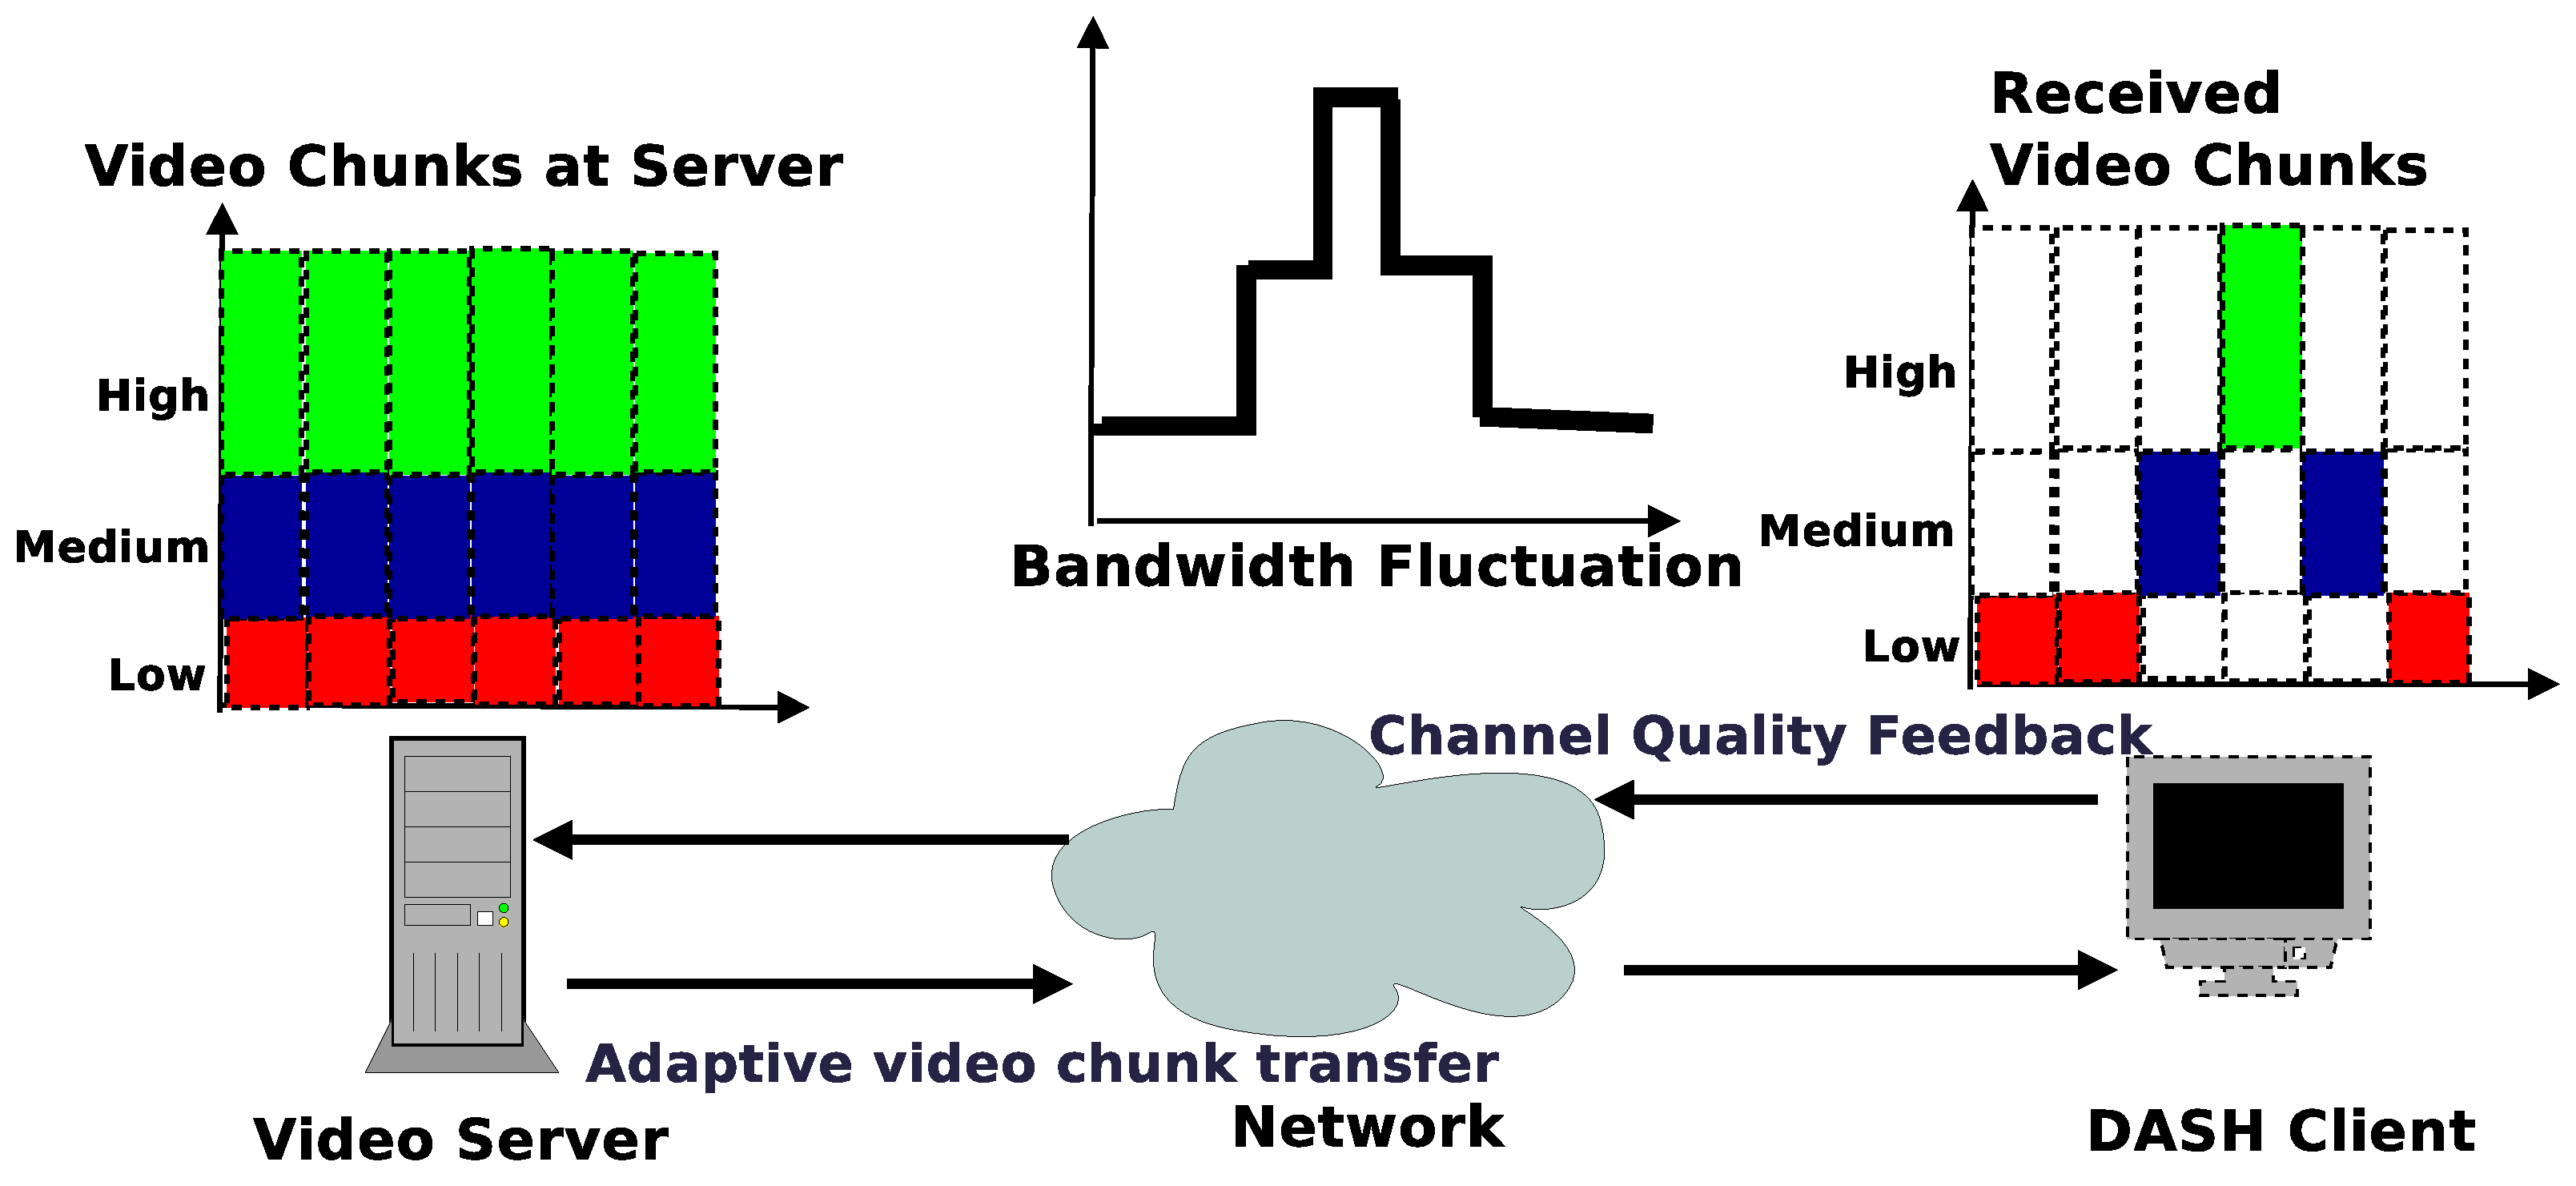
\includegraphics[width=\linewidth]{img/dash.eps}
%	\caption{\label{fig:dash}}
%\end{figure}

%The popularity of the stored video streaming (or video on demand (VOD)) led to the development of adaptive live streaming. Technology wise VOD and live streaming are not so different. In case of live streaming, all the viewer across the globe, are in sync and viewer can not seek the video. This small difference opens up an opportunity to scale the live streaming to millions of viewer with a minimal number of servers by exploiting the network between two or more nearby viewers.

%In this paper, we develop a peer-assisted collaborative live video streaming system to improve quality of experience (QoE) and reduce the bandwidth requirement and server overhead. We exploit the fact that all the live streaming viewers are in temporal sync. Almost all the viewers watch precisely the same part of the video simultaneously. So, two viewers in the proximity can collaborate in downloading the video if they are agreed to play the same quality. In our work, we find the similar video player in the proximity and make them collaborate. We develop a technique to find similar viewers in the proximity and collaborate among themselves in video playback.
